\chapter{Pandora’s Actor}

Concealed by the shadowy interior of the guest manor, Pandora’s Actor leaned against the wall of his bedroom, watching the streets below through its windows. It was a pleasant afternoon in the city, though traces of the spring rains still remained over the glistening cobblestones. A pair of Death Knights strode by on their patrol of the central district, their heavy footfalls resonating through the air. A short ways away, there was a small group of nobles which trailed behind, accompanied by their servants on their way to conduct their business somewhere. The sight was a satisfying one: proof that the efforts that had been poured into revitalizing the city and its surrounding territories were truly beginning to take hold.

 

It had been nearly three weeks since Shalltear Bloodfallen had agreed to join hands with him in his work – three weeks since the stormy night when he had been struck by the epiphany that now lay at the core of all his efforts with the citizens of the realm. He had reworked the approach by which he now encouraged the people, and reflection on his previous actions in comparison still made him chuckle ruefully to himself. He had ceased his shallow efforts to become an object of adulation; a proud figure that attempted to force the idea of bravery and resilience in all who laid eyes on him. Now, he had acted to become a constant in the eyes of the Humans, interacting with them in a much more personal manner. He was no longer just an Adventurer: he had become a friend to the people; a trusted confidante; a role model that led the citizens of the Sorcerous Kingdom into the bright future that their new sovereign had in store for them.

 

Slowly, but surely, the citizens responded to him. Through his encouragement, the people roused themselves from their fearful stupor and life returned to the duchy as inevitably as blossoms would greet the spring. The multitude of pebbles he had shifted out in the vast rural regions surrounding the city eventually turned into an avalanche. Tenants from hamlets created demand for the services of their respective villages, which in turn restarted trade and travel to and from the towns that serviced those villages. The flow of goods and labour eventually reached the capital of E-Rantel: first in a trickle, then a flood. It was startling to see how the entire city seemed to immediately come to life – as if its people had been rudely chased out of their beds by a bucket of ice water.

 

The civilization built by the Humans was both intricate and insidious in its functioning. All it had taken was a series of gentle nudges in the right places to stir it from its slumber – he had learned how to turn the key he had been given, as Shalltear had so poetically described it. As the parts of that lock tumbled and snapped into place, the people moved of their own volition to act out their roles. It seemed an irresistible thing to them: a part of their nature that they could not deny as they sought out a tiny, yet coveted position amongst their fellows. It mattered little what part they played – farmer or smith; noble or servant. All purpose was dictated by a system that had been refined over generations to suit the qualities and needs of their race. There were, of course, a few disenfranchised individuals amongst them, but they were by far a tiny minority.

 

More, he realized, had their roles supplanted by various aspects of the Sorcerous Kingdom that the Guardian Overseer saw fit to rearrange. It was something that had already come to pass and the damage had already been done, so he would need to keep an eye on things to ensure that as many as possible could partake in his Master’s vision for the realm. There was also the incorporation of the various non-human species that were already a part of the citizenry. With Humans by far the majority of the realm’s population, it seemed like the best option. The more intelligent of the nonhuman denizens would almost certainly adapt to find their place, but there were others that did not quite fit into the puzzle for one reason or another.

 

That these weak beings were not as unsophisticated and chaotic as they initially seemed was a realization that was ever so slowly dawning on the other servants of Nazarick. That they would naturally pursue higher ideals of order had struck a chord with some, and was recognized as a trait to be exploited by others. There was no doubt in his own mind that it was something long understood and incorporated into his Master’s plans: even when ruled over by one that was not of their own, they would inevitably and willingly come to embrace the order of the Sorcerous Kingdom and commit themselves fully to its cause.

 

How vast was his Creator’s intellect, knowing that not changing such a small thing would have a greater effect than a thousand alterations and amendments by the Guardian Overseer? Everything slid so naturally into place when he followed his Master’s lead, with no resistance or complaint. The work of generations shortened to mere weeks: surely one with such perfect understanding deserved to be called a Supreme Being. All there was to do now was to capitalize on this progress…but what did their Master wish of them next?

 

As he continued to ponder what his future steps would be, there was a soft knock at the door.

 

In the blink of an eye, Pandora’s Actor took on the guise of Momon, equipping the Adventurer’s dark attire. As he did so he realized it was probably unnecessary, but he completed the action regardless. He lived alone in the manor most of the time, with Narberal only occasionally frequenting it for the sake of appearances. Momon’s visitors would not be knocking at the door to this room: they would be ringing the bell to the manor and awaiting his answer outdoors.

 

“Enter,” he said.

 

Surely enough, the figure of an Eight-Edge Assassin appeared in the doorframe. It scuttled in and made a sort of bow – if such a form could be said to bow – and its mouthparts worked as it spoke.

 

“Ainz-sama has arrived to see you.”

 

Pandora’s Actor unconsciously straightened at the sound of his Master’s name.

 

“Understood. You may return.”

 

After the door closed behind the Eight-Edge Assassin, Momon’s equipment and guise vanished from Pandora’s Actor, replaced by his sharp military uniform. His fingers fidgeted nervously as they roamed to ensure his attire was impeccable. Stepping in front of a body-length mirror, he flourished his cloak for effect and evaluated the results. His cap was not straight. Or was it? He moved to adjust it carefully, then decided to tilt it, thinking it might look more dashing that way. A hand went to his chin as he pondered his image, and then he straightened his cap again.

 

His body moved from side to side, as if he could look around his reflection to catch a glimpse of himself from another angle. He rehearsed a few poses and gestures that he thought might be appropriate for a meeting with his Creator and, suitably satisfied with what he had finally settled on, Pandora’s Actor strode to the door. It would not do to keep his Master waiting.

 

As he made his way out of his room and down the stairs, he scanned the hall that encircled the courtyard, looking from door to door until he spotted the only one being guarded, which led to the drawing room of the manor. He checked over himself one last time: tilting his hat, adjusting his lapels and straightening his tie as he mentally rehearsed his actions once again before rigidly knocking at the door.

 

The door opened and he looked down to see the Homunculus Maid, Fifth. She did not meet his gaze and waited silently for him to make his entrance. Mustering all of his courage, Pandora’s Actor strode into the room grandly.

 

“Oh Supreme One!” He said boldly as his arms swept out before him, “My creator Ainz-sama–”

 

“No need to greet me. Sit.”

 

“Yes!”

 

All thoughts of his carefully rehearsed movements instantly vanished as he clicked his heels together. He goose stepped his way to the couch where the Supreme Overlord of Nazarick awaited him, and promptly seated himself. Pandora’s Actor sat stiffly as he felt his Master’s eyes closely evaluate him. Time seemed to stretch on in the silence as he did so, so he thought to fill in the space by engaging in the proper pleasantries.

 

“May I ask–”

 

“No, it’s nothing, don’t worry about it,” his Master interjected, and Pandora’s Actor immediately withdrew his words. “All right, I have some things to ask you. First, I’d like to know about Momon’s condition. I know what you’ve reported to Albedo...so, are there any problems?”

 

Aside from the die that he had cast a few weeks ago, the reports that he had given to Albedo had been, for the most part, progress reports regarding his efforts to restore the vitality of E-Rantel. The former was the only real incident that could have qualified as irregular – as the latter was the role which he had been assigned – so did that mean that his Master approved of his move to place the young noblewoman under Shalltear? He supposed it must. Surely, it must be so, considering the valuable sequence of outcomes that continued to manifest as a result, progressively branching and blossoming into a myriad of positive effects.

 

“It would seem there is nothing spec–”

 

“Is that so,” Pandora’s Actor was interrupted once again, “good. Then, I’d like to ask you, Pandora’s Actor – are there any problems on your end?”

 

It would seem that everything was going according to his Master’s plans. He relaxed somewhat, assured that his own actions had not run afoul of his Creator’s Will and pondered what sort of personal problems he might have to report. There was really only one thing – though in truth his zeal in achieving his goals had actually served as a sort of distraction from it. In truth…

 

“In truth, Ainz-sama!”

 

With the floodgates of his desire wrenched open at his Master’s prompting, the realization of what he had been missing the entire time came crashing down on him all at once.

 

“I – I have suffered greatly!”

 

As his emotions welled from within, he rose from his seat and rounded on his Master. Surely, this was an act of the kindest regard – for his Creator to be so acutely aware of his needs. He drew close, with one arm resting on the backrest of the couch and the other making animated gestures as he spoke.

 

“During this time,” Pandora’s Actor said, “I have not been able to touch magic items.”

 

Well, technically he had – though the magical conveniences of the Humans such as enchanted containers and Faucets of Spring Water were a fraction of a pittance in comparison with what lay within the vaults of Nazarick and thus did not even come close to satiating his urges.

 

“I have been unable to maintain the various magic items created by the Supreme Beings,” he continued. “The sorting of data crystals has ground to a halt as well. Please! No matter what, Ainz-sama! I beseech you to grant me some time with those items!”

 

“…I – did I design you that way?”

 

“Of that, there is no doubt!” Pandora’s Actor proclaimed, “These feelings were bestowed upon me by yourself, Momonga-sama!”

 

“Did I not permit you to return to Nazarick every day?” Momonga-sama returned after a momentary pause.

 

“But I have not received permission to return to the Treasury!”

 

Pandora’s actor returned periodically to the Great Tomb, but mainly for the purpose of creating Undead servants out of the frozen corpses on the Fifth Floor once a day. Without the Ring of Ainz Ooal Gown, which he did not carry as he travelled about the realm as Momon due to security concerns, he could not enter the hallowed sanctum of the Guild Treasury.

 

“I understand,” his Master said. “Then, I shall inform Shalltear and have her give the Ring to you. In addition, I grant you permission to work on my comrades’ weaponry and equipment. Do not damage them.”

 

The fact that he had mentioned Shalltear specifically gave Pandora’s Actor a split second’s pause. Due to their agreed-upon collaboration to achieve the ideal realm of their Master, he and the Floor Guardian kept in regular contact with one another. Did the purposeful selection mean that their Master knew well of what had transpired and had just given his tacit approval of their work? There was also the idea that she was one of the NPCs that had the Ring who could also transport herself magically, but doing so by one of the others who could not was simply a matter of asking so it must have meant the former. The thought that he had succeeded in discerning his Master’s wishes filled him with satisfaction once again.

 

He straightened his hat and rose to offer a crisp salute.

 

“It shall–”

 

“Stop that. Speaking normally will be fine. Didn’t I tell you this before, hm, Pandora’s Actor?”

 

“Yes!”

 

“The relationship between us is one of creator and created. The fact is, I am very happy with the way you have worked hard to show me the being I intended to make. However, sometimes I wonder; should children not work to exceed their parents?”

 

The fact that his work was being directly affirmed had the effect of being extremely gratifying. The idea that his Creator considered Pandora’s Actor His own child filled him with overwhelming euphoria.

 

“Ohh…Ainz-sama. To think you would refer to me as your child!”

 

“Umu, umu,” his Creator nodded. “You are…er…my son, or something like that. That, er, how shall I put this, should most likely, er, that should be the case. Therefore, there’s no need to use German or salute or be so dramatic in front of me. Since I made you, I want to see the parts of you that I did not make, as proof that you have grown.”

 

There was a sniffling sound in the background as Pandora’s Actor bowed, absorbing the edifying words from his Creator. His Creator? No…

 

“I understand – Father!”

 

“...Oh.”

 

“I shall show you what you wish to see, Father!” Pandora’s Actor declared.

 

“Pandora’s Actor. You must not tell anyone else of what has happened here. Understood? If people know that you’re receiving special treatment, it might result in friction with the others.” His Father’s voice was solem, “Also – in fact, because of that, I will be placing you lower on my priorities. If the time comes when I have to choose between helping you or the Floor Guardians, I will abandon you.”

 

It felt something of a relief that he was least on the list of his Father’s concerns. The vote of confidence filled him with pride, and he thrust out his chest after he rose to stand tall.

 

“But of course! Please, sacrifice me as you see fit!”

 

“I am sorry. And...Fifth. Do not speak of what has happened here.”

 

The Homunculus Maid attending to their Master nodded in acknowledgement of the order. Ainz Ooal Gown rose from his seat with a regal nod.

 

“Then, I will be on my way.”

 

Understanding that absolutely no one was to know of their meeting, Pandora’s Actor locked away the precious memory in the treasury of his heart. He was now supremely assured that his work was as his Father had wished of him. The Supreme Overlord of Nazarick knew what Pandora’s Actor had been doing, and had visited to personally deliver his approval. Still, there were many questions that lingered in his mind: questions which echoed in the voices of the people that he had become much more than just a hero to. He thought of the humble families of tenant labourers in their rural lands; of the craftsmen and shopkeepers in the settlements that they serviced; of the nobles who administered their fiefs and pioneered the new ways that would become the foundations of the Sorcerous Kingdom.

 

“Ah, about that,” he felt compelled to speak before they parted ways, “could you hold on a little? Since we meet rarely, there is a matter that I would like to ask you, Father.”

 

Since his Father had stated that he would now be focusing more on the others, Pandora’s Actor seized the opportunity to ask on the peoples’ behalf.

“May I know how you intend to rule this Sorcerous Kingdom?”

\section*{End of Act Character Sheets}

\begin{figure}
    \centering
    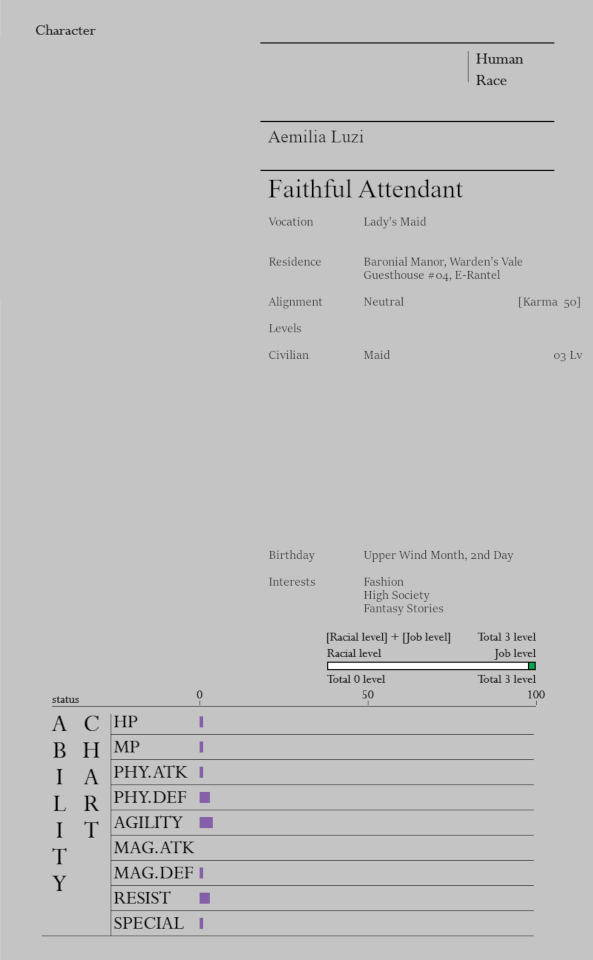
\includegraphics[width=1\textwidth]{images/q0TuUBL.png}
    \caption*{Aemilia Luzi Character Sheet - Act 3}
\end{figure}

\begin{figure}
    \centering
    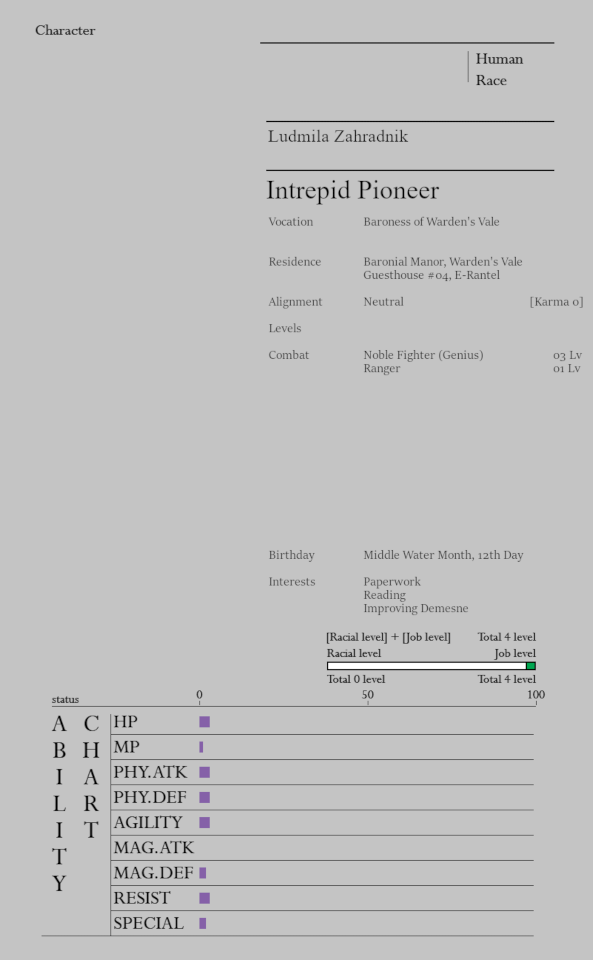
\includegraphics[width=1\textwidth]{images/Rzh3Deu.png}
    \caption*{Ludmila Zahradnik Character Sheet - Act 3}
\end{figure}
